% Disabled the use of Source Code Pro -- problems with scaled fonts (trh 24/8/2019)
% This allowed the user manual to build using pdflatex and latex
\documentclass[letter]{article}
\usepackage{fancyhdr} % Required for custom headers
\usepackage{lastpage} % Required to determine the last page for the footer
\usepackage{extramarks} % Required for headers and footers
\usepackage[usenames,dvipsnames]{color} % Required for custom colors
\usepackage[table]{xcolor}
\usepackage{graphicx} % Required to insert images
\usepackage{listings} % Required for insertion of code
\usepackage{algpseudocode} % Required for pseudocode listing
\usepackage{courier} % Required for the courier font
\usepackage{amsmath}
\usepackage{amssymb}
\usepackage{booktabs}
\usepackage{multirow}
\usepackage{tikz}
\usetikzlibrary{arrows, shapes, positioning, calc}
\usepackage{caption}
\usepackage{wasysym}
\usepackage{multirow}
\usepackage{float}
\usepackage{tcolorbox}
\usepackage{csquotes}
\usepackage{fancybox}
\usepackage{enumitem}
\usepackage[letterspace=150]{microtype}
\usepackage{cancel}
\usepackage{bm}
\usepackage{makeidx}
\usepackage{url}
\usepackage[pdfborder={0 0 0}]{hyperref}

% Disabled the use of Source Code Pro -- problems with scaled fonts (trh 24/8/2019)
%\usepackage{sourcecodepro}

\definecolor{MyDarkGreen}{rgb}{0.0,0.4,0.0} % This is the color used for comments
\definecolor{mygreen}{rgb}{0,0.6,0}
\definecolor{mygray}{rgb}{0.5,0.5,0.5}
\definecolor{mymauve}{rgb}{0.58,0,0.82}

\lstset{ %
  backgroundcolor=\color{white},   % choose the background color; you must add \usepackage{color} or \usepackage{xcolor}
% Disabled the use of Source Code Pro -- problems with scaled fonts (trh 24/8/2019)
% basicstyle=\sourcecodepro\footnotesize ,        % the size of the fonts that are used for the code
  basicstyle=\footnotesize ,        % the size of the fonts that are used for the code
  breakatwhitespace=true,         % sets if automatic breaks should only happen at whitespace
  breaklines=true,                 % sets automatic line breaking
  captionpos=b,                    % sets the caption-position to bottom
  commentstyle=\color{mygreen},    % comment style
  deletekeywords={...},            % if you want to delete keywords from the given language
  escapeinside={(*}{*)},          % if you want to add LaTeX within your code
  extendedchars=true,              % lets you use non-ASCII characters; for 8-bits encodings only, does not work with UTF-8
  frame=single,                    % adds a frame around the code
  keepspaces=true,                 % keeps spaces in text, useful for keeping indentation of code (possibly needs columns=flexible)
  keywordstyle=\color{blue},       % keyword style
  language=C,                 % the language of the code
  morekeywords={repeat,integer,function,end,*,...},            % if you want to add more keywords to the set
  numbers=left,                    % where to put the line-numbers; possible values are (none, left, right)
  numbersep=5pt,                   % how far the line-numbers are from the code
  numberstyle=\tiny\color{mygray}, % the style that is used for the line-numbers
  rulecolor=\color{black},         % if not set, the frame-color may be changed on line-breaks within not-black text (e.g. comments (green here))
  showspaces=false,                % show spaces everywhere adding particular underscores; it overrides 'showstringspaces'
  showstringspaces=false,          % underline spaces within strings only
  showtabs=false,                  % show tabs within strings adding particular underscores
  stepnumber=1,                    % the step between two line-numbers. If it's 1, each line will be numbered
  stringstyle=\color{mymauve},     % string literal style
  tabsize=2,                       % sets default tabsize to 2 spaces
  title=\lstname                   % show the filename of files included with \lstinputlisting; also try caption instead of title
}


% Margins
\topmargin=-0.45in
\evensidemargin=0in
\oddsidemargin=0in
\textwidth=6.5in
%\textheight=9.0in
\headsep=0.25in

\linespread{1.1} % Line spacing

% Set up the header and footer
%\pagestyle{fancy}
%\renewcommand\headrulewidth{0.4pt} % Size of the header rule
%\renewcommand\footrulewidth{0.4pt} % Size of the footer rule

\setlength\parindent{0pt} % Removes all indentation from paragraphs

\renewcommand{\familydefault}{\sfdefault}

\newcommand{\mb}[1]{{\bf{#1}}}
\newcommand{\tr}{^{\sf T}}

\title{Mongoose User Guide, Version 2.0.4}
\author{Scott Kolodziej, Nuri Yeralan, Tim Davis, William W. Hager}
\date{May 25, 2019}


\makeindex

\begin{document}

\maketitle

\tableofcontents

\newpage

\section{Overview}
% What is the problem we're solving? What does this package do?
Mongoose is a graph partitioning library that can quickly compute edge cuts in arbitrary graphs \cite{MongooseTOMS}. Given a graph with a vertex set $V$ and edge set $E$, an edge cut is a partitioning of the graph into two subgraphs that are balanced (contain the same number of vertices) and the connectivity between the subgraphs is minimized (few edges are in the cut).
\\

Finding high quality edge cuts quickly is an important part of circuit simulation, parallel and distributed computing, and sparse matrix algorithms.

\subsection{Coarsening and Refinement Framework}

Mongoose uses a coarsening and refinement framework (sometimes referred to as a multilevel framework \cite{HendricksonLeland1995, KarypisKumar1995}). Rather than attempt to compute an edge cut on the input graph directly, Mongoose first coarsens the graph by computing a vertex matching and contracting the graph to form a smaller, but structurally similar, graph.

\begin{figure}[!ht] 
\begin{center} 
    \includegraphics[scale=0.18]{Figures/MultilevelOverview.eps} 
    \caption{Coarsening and Refinement} 
\end{center} 
\end{figure} 

Mongoose uses a variety of methods to coarsen the input graph, including random matching and heavy-edge matching. Additionally, Mongoose offers stall-reducing vertex matching strategies called Brotherly (or two-hop) matching and Community matching. Brotherly matching allows vertices who share a neighbor to be matched, even if they have no edge directly connecting them, and community matching allows two vertices whose neighbors are matched together to be matched together. These methods are advantageous in efficiently coarsening certain classes of graphs, notably social networking graphs, where the vertex degree can vary greatly.

\begin{center}
\begin{minipage}[c]{0.47\linewidth}
    \includegraphics[scale=0.26]{Figures/BrotherlyMatching.eps} 
    \captionof{figure}{Brotherly Matching} 
\end{minipage}
\hspace{22pt}
\begin{minipage}[c]{0.47\linewidth}
    \includegraphics[scale=0.26]{Figures/CommunityMatching.eps} 
    \captionof{figure}{Community Matching} 
\end{minipage}
\end{center}

Another matching strategy used in Mongoose is known as Adoption matching. If an unmatched vertex has no unmatched neighbors, it can be grouped into a 3-way matching with a neighboring matched vertex. These strategies allow the graph to be coarsened quickly even when the graph is highly irregular, which in turn decreases memory requirements and overall computational time.

\subsection{Quadratic Programming and Optimization}

Mongoose is known as a hybrid graph partitioner, as it uses multiple methods in tandem to find higher quality cuts efficiently. The first such method Mongoose employs is quadratic programming (QP). The edge cut problem was formatted as a continuous quadratic programming problem by Hager and Krylyuk \cite{HagerKrylyuk1999}. This formulation is solved (rather, improved) using a gradient projection algorithm and a modified version of NAPHEAP, a quadratic knapsack solver \cite{DavisHagerHungerford2016}.
\\

The quadratic program used is shown below. Hager and Krylyuk have proven that the global optimum to this quadratic program yields the solution to the graph partitioning problem (but note that both are NP-hard problems to solve).
%
\begin{eqnarray}
&\displaystyle\min_{\mb{x}\in\mathbb{R}^n}\quad  (\mb{1} - \mb{x})\tr (\mb{A} + \mb{I})\mb{x}
& \quad \mbox{subject to}  \quad
\mb{0} \le \mb{x} \le \mb{1}, \quad \ell \le \mb{1}\tr \mb{x} \le u, \nonumber
\end{eqnarray}

$\ell$ and $u$ are lower and upper bounds on the desired size of one partition, and $\mb{A}$ is the adjacency matrix of the graph.

\subsection{Fiduccia-Mattheyses Algorithm}

In addition to the quadratic programming approach for refining an edge cut, a standard implementation of the Fiduccia-Mattheyses algorithm \cite{FiducciaMattheyses1982} is also provided. This involves swapping vertices from one part to the other in an effort to improve the edge cut quality. Some vertices are swapped even if no immediate improvement is found in an attempt to escape a locally optimal solution. However, if no improvement is found after a number of swaps, the change is reverted.\\
\\
The Fiduccia-Mattheyses (FM) implementation in Mongoose utilizes heaps for high efficiency. 

\section{Availability}

\subsection{Getting the Code}
Mongoose is available on GitHub at \url{https://github.com/ScottKolo/Mongoose}. The code can be downloaded using \texttt{git} using the following command:
\[\text{\texttt{git clone https://github.com/ScottKolo/Mongoose}}\]
Alternatively, Mongoose can be downloaded as a zip archive from the following URL:
\[\text{\url{https://github.com/ScottKolo/Mongoose/archive/edgesep.zip}}\] 

Mongoose also appears as a component package of SuiteSparse, \url{http://suitesparse.com}.

\subsection{Prerequisites}
Mongoose requires CMake 2.8 and any ISO/IEC 14882:1998 compliant C++ compiler. Mongoose has been tested to work with GNU GCC 4.4+ and LLVM Clang 3.5+ on Linux, and Apple Xcode 6.4+ on macOS.

\subsection{Compilation}
Once downloaded, Mongoose can be compiled using the following commands:\\

\begin{lstlisting}[language=bash,numbers=none,xleftmargin=.2\textwidth, xrightmargin=.2\textwidth]
cd Mongoose
make
\end{lstlisting}

% mkdir build # Create a build directory
% cd build 
% cmake ..     # Use CMake to create the Makefiles
% make         # Build Mongoose

After compilation, the Mongoose demo can be run using \texttt{./bin/demo}:\\

\begin{lstlisting}[numbers=none,xleftmargin=.09\textwidth, xrightmargin=.09\textwidth,keywordstyle=\color{black}]
./bin/demo

********************************************************************************
Mongoose Graph Partitioning Library, Version 2.0.2 July 5, 2018
Copyright (C) 2017-2018
Scott P. Kolodziej, Nuri S. Yeralan, Timothy A. Davis, William W. Hager
Mongoose is licensed under Version 3 of the GNU General Public License.
Mongoose is also available under other licenses; contact authors for details.
********************************************************************************
Computing an edge cut for Erdos971.mtx...
Cut Cost:       1.1e+02
Cut Imbalance:  zero (a perfect balance)
Trial Time:     1.9ms
********************************************************************************
Computing an edge cut for G51.mtx...
Cut Cost:       1.5e+03
Cut Imbalance:  zero (a perfect balance)
Trial Time:     8.4ms
********************************************************************************
Computing an edge cut for GD97_b.mtx...
Cut Cost:       2.6e+03
Cut Imbalance:  1.1%
Trial Time:     0.19ms
********************************************************************************
Computing an edge cut for Pd.mtx...
Cut Cost:       1
Cut Imbalance:  0.0062%
Trial Time:     12ms
********************************************************************************
Computing an edge cut for bcspwr01.mtx...
Cut Cost:       3
Cut Imbalance:  1.3%
Trial Time:     0.18ms
********************************************************************************
Computing an edge cut for bcspwr02.mtx...
Cut Cost:       5
Cut Imbalance:  1%
Trial Time:     0.17ms
********************************************************************************
Computing an edge cut for bcspwr03.mtx...
Cut Cost:       11
Cut Imbalance:  zero (a perfect balance)
Trial Time:     0.34ms
********************************************************************************
Computing an edge cut for bcspwr04.mtx...
Cut Cost:       25
Cut Imbalance:  zero (a perfect balance)
Trial Time:     0.75ms
********************************************************************************
Computing an edge cut for bcspwr05.mtx...
Cut Cost:       12
Cut Imbalance:  0.11%
Trial Time:     0.91ms
********************************************************************************
Computing an edge cut for bcspwr06.mtx...
Cut Cost:       7
Cut Imbalance:  zero (a perfect balance)
Trial Time:     2.4ms
********************************************************************************
Computing an edge cut for bcspwr07.mtx...
Cut Cost:       7
Cut Imbalance:  zero (a perfect balance)
Trial Time:     2.6ms
********************************************************************************
Computing an edge cut for bcspwr08.mtx...
Cut Cost:       25
Cut Imbalance:  zero (a perfect balance)
Trial Time:     2.2ms
********************************************************************************
Computing an edge cut for bcspwr09.mtx...
Cut Cost:       11
Cut Imbalance:  0.029%
Trial Time:     5.4ms
********************************************************************************
Computing an edge cut for bcspwr10.mtx...
Cut Cost:       25
Cut Imbalance:  zero (a perfect balance)
Trial Time:     8.6ms
********************************************************************************
Computing an edge cut for dwt_992.mtx...
Cut Cost:       1.9e+02
Cut Imbalance:  zero (a perfect balance)
Trial Time:     4.7ms
********************************************************************************
Computing an edge cut for jagmesh7.mtx...
Cut Cost:       27
Cut Imbalance:  zero (a perfect balance)
Trial Time:     2.8ms
********************************************************************************
Computing an edge cut for NotreDame_www.mtx...
Cut Cost:       1.9e+02
Cut Imbalance:  0.00015%
Trial Time:     6.2e+02ms
********************************************************************************
Total Demo Time:  0.67s

Demo complete; all tests passed
\end{lstlisting}

To run the complete test suite, the command \texttt{make test} can be used. Note that Python 2.7+ must be installed. Additionally, this user guide can be generated from source with the command \texttt{make userguide}. XeLaTeX (commonly included in LaTeX distributions) must be installed.

\section{Using Mongoose as an Executable}

In addition to the demo executable, the \texttt{mongoose} executable is built at \texttt{./bin/mongoose}. This executable can be used to partition a graph given a Matrix Market file:

\[\text{\texttt{mongoose <MM-input-file.mtx> [output-file]}}\]

The \texttt{mongoose} executable generates a text file with two blocks: a JSON-formatted information block with timing and cut quality metrics, and the partitioning information itself. The partitioning information is listed with one vertex per line, with the vertex number followed by the part (0 for part A, 1 for part B).\\

For example, the following can be used to partition the \texttt{NotreDame\_www.mtx} matrix:

\begin{lstlisting}[numbers=none,xleftmargin=.09\textwidth, xrightmargin=.09\textwidth,keywordstyle=\color{black}]
cd build
./bin/mongoose ../Matrix/NotreDame_www.mtx NotreDame_www_out.mtx

********************************************************************************
Mongoose Graph Partitioning Library, Version 2.0.2 July 5, 2018
Copyright (C) 2017-2018
Scott P. Kolodziej, Nuri S. Yeralan, Timothy A. Davis, William W. Hager
Mongoose is licensed under Version 3 of the GNU General Public License.
Mongoose is also available under other licenses; contact authors for details.
********************************************************************************
Total Edge Separator Time: 0.256587s
 Matching:   0.03576s
 Coarsening: 0.05597s
 Refinement: 0.01149s
 FM:         0.002221s
 QP:         0.1448s
 IO:         0.3147s
Cut Properties:
 Cut Size:       320
 Cut Cost:       165
 Imbalance:      1.535e-06
\end{lstlisting}

The output file name is optional. If omitted, the default is \texttt{mongoose\_out.txt}.
For this matrix, the output file looks like the following:

\begin{lstlisting}[numbers=none,xleftmargin=.09\textwidth, xrightmargin=.09\textwidth,keywordstyle=\color{black}]
{
  "InputFile": "../Matrix/NotreDame_www.mtx",
  "Timing": {
    "Total": 0.256587,
    "Matching": 0.035762,
    "Coarsening": 0.055973,
    "Refinement": 0.011487,
    "FM": 0.002221,
    "QP": 0.144759,
    "IO": 0.314704
  },
  "CutSize": 320,
  "CutCost": 165,
  "Imbalance": 1.53502e-06
}

0 0
1 0
2 0
3 0
...
218 1
219 0
...
325660 1
325661 1
325662 1
325664 0
325665 0
...
325727 0
325728 0

\end{lstlisting}

\subsection{License}

Mongoose is licensed under the GNU Public License version 3 (GPLv3). Full text of the license can be found int \texttt{Mongoose/Doc/License.txt}. For a commercial license, please contact Dr.~Timothy A.~Davis at davis@tamu.edu.

\section{Using Mongoose in C++}

\subsection{Sample C++ Program}
% Without weights, with edge weights, with vertex weights

\begin{lstlisting}
#include "Mongoose.hpp"
#include <iostream>
#include <iomanip>
#include <math.h>

using namespace Mongoose;
using namespace std;

int main(int argn, const char **argv)
{
    EdgeCut_Options *options = EdgeCut_Options::create();
    if (!options) return EXIT_FAILURE; // Return an error if we failed.

    options->matching_strategy = HEMSRdeg;
    options->initial_cut_type = InitialEdgeCut_QP;

    Graph *graph = read_graph(argv[1]);
    if (!graph)
    {
        options->~EdgeCut_Options();
        return EXIT_FAILURE;
    }

    // Call Mongoose to compute an edge separator
    EdgeCut *result = edge_cut(graph, options);

    cout << "Partitioning Complete!" << endl;
    cout << "Cut Cost:      " << setprecision(2) << result->cut_cost << endl;
    cout << "Cut Imbalance: " << setprecision(2) << fabs(100*result->imbalance) << "%" << endl;

    options->~EdgeCut_Options();
    graph->~Graph();
    result->~EdgeCut();

    /* Return success */
    return EXIT_SUCCESS;
}
\end{lstlisting}

\subsection{Creating a Graph}

There are several different ways to create a \texttt{Graph} class instance for use in Mongoose.

The input graph to Mongoose is undirected, and can optionally be a weighted
graph.  The graph is held in compressed-sparse column form, or equivalently
compressed-sparse row form since the adjacency matrix is symmetric.  The graph
is represented by the following components:

    \begin{itemize}
    \item \texttt{Int n}: the number of vertices in the graph.
    \item \texttt{Int nz}: the number of nonzero entries in the adjacency matrix,
        which is twice the number edges.
    \item \texttt{Int p [n+1]}: the column pointer vector of size \texttt{n+1}.
    \item \texttt{Int i [nz]}: the adjacency lists held in a single array.  The adjacency
        list of vertex \texttt{j} is held in \texttt{i [p [j] ... p [j+1]-1]}.
        Self-edges must not appear.
        The graph must be undirected, and so the adjacency matrix must be symmetric.
    \item \texttt{double x [nz]}: an optional array of edge weights, where
        \texttt{x [p [j] ... p [j+1]-1]} are the edge weights of the corresponding
        edges in the adjacency list of vertex \texttt{j}.
        If \texttt{x} is \texttt{NULL}, then the edges all have weight 1.
    \item \texttt{double w [n]}: an optional array of vertex weights,
        where vertex \texttt{j} has weight \texttt{w [j]}.
        If \texttt{w} is \texttt{NULL}, then the vertices all have weight 1.
    \end{itemize}
    
Note that the \texttt{Int} type is generally a 64-bit (long) integer type. It is defined as \texttt{typedef SuiteSparse\_long Int;} which is further defined as \texttt{\#define SuiteSparse\_long long} in SuiteSparse\_config.

\subsubsection{Creating a Graph Manually}

To create a graph manually, the following constructor is used: \\

\textbf{\texttt{static Graph *create(const Int \_n, \\
\hspace*{4.2cm} const Int \_nz, \\
\hspace*{4.2cm} Int *\_p = NULL, \\
\hspace*{4.2cm} Int *\_i = NULL, \\
\hspace*{4.2cm} double *\_x = NULL, \\
\hspace*{4.2cm} double *\_w = NULL);}}\\
\\
Using the manual constructor, the number of vertices (or dimension of the matrix, \texttt{Int \_n}) and the number of edges (or nonzero entries in the matrix, \texttt{Int \_nz}) must both be specified. The column pointer vector \texttt{Int *\_p} and row index vector \texttt{Int *\_i} must either be specified by the user, or, if left \texttt{NULL}, they will be allocated such that \texttt{\_p = (Int *)SuiteSparse\_calloc(n + 1, sizeof(Int));} and \texttt{\_i = (Int *)SuiteSparse\_malloc(nz, sizeof(Int));}. The edge weights \texttt{double *\_x} and the vertex weights \texttt{double *\_w} can either be specified, or, if left \texttt{NULL}, will be assumed to be one for all edges and vertices, respectively.\\

Here are some examples:

\begin{itemize}
\item \texttt{Graph::create(20, 50);} creates a \texttt{Graph} with 20 vertices and 50 edges, but no data. \texttt{Graph->p} and \texttt{Graph->i} are allocated by Mongoose to store exactly 20 columns (vertices) and 50 nonzero elements (edges). This allows the user to populate \texttt{Graph->p} and \texttt{Graph->i} manually. All edge and vertex weights are assumed to be one.
\item \texttt{Graph::create(20, 50, \_p, \_i);} creates a \texttt{Graph} with 20 vertices and 50 edges with the pattern specified. \texttt{Graph->p} and \texttt{Graph->i} are shallow copies of the arguments \texttt{\_p} and \texttt{\_i} and will not be freed upon calling the destructor. All edge and vertex weights are assumed to be one.
\item \texttt{Graph::create(20, 50, \_p, \_i, \_x);} creates a \texttt{Graph} with 20 vertices and 50 edges with the pattern and edge weights specified. \texttt{Graph->p}, \texttt{Graph->i}, and \texttt{Graph->x} are shallow copies of the arguments \texttt{\_p}, \texttt{\_i}, and \texttt{\_x}, and will not be freed upon calling the destructor. Edge weights are specified by \texttt{\_x}, but vertex weights are assumed to be one.
\item \texttt{Graph::create(20, 50, \_p, \_i, \_x, \_w);} creates a \texttt{Graph} with 20 vertices and 50 edges with edge and vertex weights specified. \texttt{Graph->p}, \texttt{Graph->i}, \texttt{Graph->x}, and \texttt{Graph->w} are shallow copies of the arguments \texttt{\_p}, \texttt{\_i}, \texttt{\_x}, and \texttt{\_w}, and will not be freed upon calling the destructor. Edge weights are specified by \texttt{\_x}, and vertex weights are specified by \texttt{\_w}.
\end{itemize}


\subsubsection{Creating a Graph from a Sparse Matrix}

Another way to create a \texttt{Mongoose::Graph} is from a pre-existing \texttt{CSparse} matrix struct.\\

\textbf{\texttt{static Graph *Create(cs *matrix);}}\\

Using this constructor, a \texttt{CSparse} matrix struct can be passed directly, with shallow copies made of \texttt{cs->p}, \texttt{cs->i}, and \texttt{cs->x}. Note that  this constructor is equivalent to calling the following for a \texttt{CSparse} matrix \texttt{cs *A}:\\

\textbf{\texttt{Graph::create(const Int A->n, A->p[A->n], A->p, A->i, A->x, NULL);}}

\subsubsection{Creating a Graph from a Matrix Market File}

Perhaps the easiest way to create a \texttt{Graph} instance is from a file. Mongoose provides easy file input helpers to read, sanitize, and format a Matrix Market file. The matrix contained in the file must be sparse, real, and square. If the matrix is not symmetric, it will be made symmetric by computing $\frac{1}{2}(A+A^T)$. If a diagonal is present, it will be removed.\\

\textbf{\texttt{Graph *read\_graph(const std::string \&filename);}}\\
\textbf{\texttt{Graph *read\_graph(const char *filename);}}\\

For example, to read in the Matrix Market file \texttt{jagmesh7.mtx} located in the Mongoose sample matrix directory, the following code can be used:\\

\textbf{\texttt{Mongoose::read\_graph(``../Matrix/jagmesh7.mtx");}}

\subsection{C++ API}

The following functions are available in the C++ API. After Mongoose is compiled, a static library version of Mongoose is built at \texttt{Mongoose/build/Lib/libmongoose.a}. Include the \texttt{Mongoose.hpp} header file located in \texttt{Mongoose/Include} and link with the static library to enable the following API functions.
Both the static and dynamic libraries, and the include file can then be
installed for system-wide use with \texttt{sudo make install} in the top-level
\texttt{Mongoose} directory.

\begin{itemize}
\item \textbf{\texttt{Graph *read\_graph(const std::string \&filename);}} \vspace{-6pt}
\item \textbf{\texttt{Graph *read\_graph(const char *filename);}}

\texttt{Mongoose::read\_graph} will attempt to read a Matrix Market file with the given filename and convert it to a Mongoose Graph instance. The matrix contained in the file must be sparse, real, and square. If the matrix is not symmetric, it will be made symmetric by computing $\frac{1}{2}(A+A^T)$. If a diagonal is present, it will be removed.

\texttt{Mongoose::read\_graph(const std::string \&filename)} accepts a C++-style std::string, while \texttt{Mongoose::read\_graph(const char *filename)} accepts a C-style null-terminated string.
\vspace{6pt}
\item \textbf{\texttt{EdgeCut edge\_cut(const Graph *);}} \vspace{-6pt}
\item \textbf{\texttt{EdgeCut edge\_cut(const Graph *, const EdgeCut\_Options *);}}

\texttt{Mongoose::edge\_cut} will attempt to compute an edge cut of the provided \texttt{Mongoose::Graph} object. An \texttt{EdgeCut\_Options} struct can also be supplied to modify how the edge cut is computed -- otherwise, the default options are used (see Section \ref{sec:options}). The resulting partitioning information is returned as an \texttt{EdgeCut} struct.

The \texttt{EdgeCut} struct is shown below.

\begin{lstlisting}
struct EdgeCut
{
    bool *partition;     /** T/F denoting partition side     */
    Int n;               /** # vertices                      */

    /** Cut Cost Metrics *****************************************************/
    double cut_cost;    /** Sum of edge weights in cut set    */
    Int cut_size;       /** Number of edges in cut set        */
    double w0;          /** Sum of partition 0 vertex weights */
    double w1;          /** Sum of partition 1 vertex weights */
    double imbalance;   /** Degree to which the partitioning
                            is imbalanced, and this is
                            computed as (0.5 - w0/W).         */

    // Destructor
    ~EdgeCut();
};
\end{lstlisting}

\vspace{6pt}
\item \textbf{\texttt{static EdgeCut\_Options *create();}}

\texttt{Mongoose::EdgeCut\_Options::create} will return an \texttt{EdgeCut\_Options} struct with default state (see Section \ref{sec:options} for details about option fields and defaults). To run Mongoose with specific options, call \texttt{EdgeCut\_Options::create} and modify the struct as needed.
\vspace{6pt}
\item \textbf{\texttt{static Graph *create(const Int \_n, \\
\hspace*{4.2cm} const Int \_nz, \\
\hspace*{4.2cm} Int *\_p = NULL, \\
\hspace*{4.2cm} Int *\_i = NULL, \\
\hspace*{4.2cm} double *\_x = NULL, \\
\hspace*{4.2cm} double *\_w = NULL);}}
\item \textbf{\texttt{static Graph *create(cs *matrix);}}

\texttt{Mongoose::Graph::create} is the primary constructor for the \texttt{Graph} class. There are two versions: one to manually specify attributes of the \texttt{Graph}, and one to form a \texttt{Graph} from a \texttt{CSparse} struct.

Using the manual constructor, the number of vertices (or dimension of the matrix, \texttt{Int \_n}) and the number of edges (or nonzero entries in the matrix, \texttt{Int \_nz}) must both be specified. The column pointer vector \texttt{Int *\_p} and row index vector \texttt{Int *\_i} must either be specified by the user, or, if left \texttt{NULL}, they will be allocated such that \texttt{\_p = (Int *)SuiteSparse\_calloc(n + 1, sizeof(Int));} and \texttt{\_i = (Int *)SuiteSparse\_malloc(nz, sizeof(Int));}. The edge weights \texttt{double *\_x} and the vertex weights \texttt{double *\_w} can either be specified, or, if left \texttt{NULL}, will be assumed to be one for all edges and vertices, respectively.

Note that Mongoose will NOT free pointers passed to it, and that all pointers are shallow copies (i.e. Mongoose does not make a copy of any data passed into it).

\vspace{6pt}
\item \textbf{\texttt{$\sim$EdgeCut\_Options();}} is the destructor for the \texttt{EdgeCut\_Options} struct. If the user creates an \texttt{EdgeCut\_Options} struct using \texttt{EdgeCut\_Options::create}, the user is also responsible for destructing it.
\item \textbf{\texttt{$\sim$Graph();}} is the destructor for the \texttt{Graph} class. If the user creates a \texttt{Graph} class instance using \texttt{Graph::create}, the user is also responsible for destructing it.
\item \textbf{\texttt{$\sim$EdgeCut();}} is the destructor for the \texttt{EdgeCut} struct. After calling \texttt{edge\_cut()}, the returned struct must be destructed when the user is finished reading data from it.
\end{itemize}

\subsection{A Note on Memory Management}

Mongoose uses three primary data structures to pass information: the \texttt{Graph} class, the \texttt{EdgeCut} struct, and the \texttt{EdgeCut\_Options} struct. They are all dynamically allocated and must be destructed.

\begin{itemize}
\item For each \texttt{Graph::create}, there should be a matching \texttt{Graph::$\sim$Graph()}.
\item For each \texttt{EdgeCut\_Options::create}, there should be a matching \texttt{EdgeCut\_Options::$\sim$EdgeCut\_Options()};
\item For each call to \texttt{edge\_cut}, there should be a matching \texttt{EdgeCut::$\sim$EdgeCut()};
\end{itemize}

Lastly, Mongoose will NOT free pointers passed to it, and that all pointers are shallow copies (i.e. Mongoose does not make a copy of any data passed into it). Freeing memory referenced by Mongoose prior to Mongoose completing will result in a segmentation fault.

\section{Using Mongoose in MATLAB}

\subsection{To Install the MATLAB Interface}

To compile Mongoose for MATLAB, go to the \texttt{MATLAB} directory and type
\texttt{mongoose\_make} in the MATLAB command window.  Be sure to use a
compiler supported by MATLAB.  Type \texttt{doc mex} in MATLAB, or visit
\url{https://www.mathworks.com/support/compilers.html} for details.  For
example, GCC 5.5.0 on Linux is not supported by MATLAB R2017A, and it will not
successfully compile Mongoose for that version of MATLAB.  MATLAB R2018b
supports GCC 6.3.x on Linux.

\subsection{Sample MATLAB Program}

Below is a sample MATLAB program using the Mongoose MATLAB API. First, it loads in a matrix, sanitizes it, and then partitions it using edge and vertex weights, then only edge weights, and the no weights.

\begin{lstlisting}[language=MATLAB]
% A simple demo to demonstrate Mongoose. Reads in a matrix, sanitizes it,
% and partitions it several different ways.
function mongoose_demo

% Obtain the adjacency matrix
matfile_data = matfile('494_bus.mat');
Prob = matfile_data.Problem;
A = Prob.A;
[m ~] = size(A);

% Sanitize the adjacency matrix: remove diagonal elements, make edge weights 
% positive, and make sure it is symmetric. If the matrix is not symmetric 
% or square, a symmetric matrix (A+A')/2 is built.
A = sanitize(A);

% Create a vertex weight vector and create a heavy vertex
V = ones(1,m);
V(10) = 300;

% Create a set of default options and modify the target balance
O = edgecut_options();
O.target_split = 0.3;

% Run Mongoose to partition the graph with edge and vertex weights.
partVert = edgecut(A, O, V);

fprintf('\n\nPartitioning graph with edge and vertex weights\n\n');
fprintf('=== Cut Info ===\n');
fprintf('Cut Size:   %d\n', full(sum(partVert .* sum(sign(A)))));
fprintf('Cut Weight: %d\n\n', full(sum(partVert .* sum(A))));
fprintf('=== Balance Info ===\n');
fprintf('Target Split:     0.3\n');
fprintf('Actual Split:     %1.4f\n', sum(partVert .* V) / sum(V));
fprintf('Unweighted Split: %1.4f\n', sum(partVert) / m);

% Run Mongoose to partition the graph with no vertex weights.

partEdge = edgecut(A, O);

fprintf('\n\nPartitioning graph with only edge weights\n\n');
fprintf('=== Cut Info ===\n');
fprintf('Cut Size:   %d\n', full(sum(partEdge .* sum(sign(A)))));
fprintf('Cut Weight: %d\n\n', full(sum(partEdge .* sum(A))));
fprintf('=== Balance Info ===\n');
fprintf('Target Split: 0.5\n');
fprintf('Actual Split: %1.4f\n', sum(partEdge) / m);

% Remove edge weights
A = sanitize(A, 1);

% Run Mongoose to partition the graph with no edge weights.
% Note that only the graph is passed as an argument, so default
% options are assumed.
partPattern = edgecut(A);

fprintf('\n\nPartitioning graph with only edge weights\n\n');
fprintf('=== Cut Info ===\n');
fprintf('Cut Size:   %d\n', full(sum(partPattern .* sum(sign(A)))));
fprintf('Cut Weight: %d\n\n', full(sum(partPattern .* sum(A))));
fprintf('=== Balance Info ===\n');
fprintf('Target Split: 0.5\n');
fprintf('Actual Split: %1.4f\n', sum(partPattern) / m);

figure('Position', [100, 100, 1000, 400]);

% Plot the original matrix before permutation
subplot(1, 2, 1);
spy(A)
title('Before Partitioning')

% Plot the matrix after the permutation
subplot(1, 2, 2);
perm = [find(partEdge) find(1-partEdge)];
A_perm = A(perm, perm); % Permute the matrix
spy(A_perm)
title('After Partitioning')

% Set overall title
suptitle('HB/494\_bus')

end
\end{lstlisting}

\subsection{MATLAB API}

\begin{itemize}
\item \textbf{\texttt{function [G\_coarse, A\_coarse, map] = coarsen (G, \textit{Opts}, \textit{A})}}\\
\texttt{coarsen} is used to coarsen an adjacency matrix (\texttt{G}) one level (one round of matching). An optional edgecut\_options struct (\texttt{Opts}) can be specified, as well as vertex weights (\texttt{A}).
\\
\item \textbf{\texttt{function options = edgecut\_options()}}\\
\texttt{edgecut\_options()} returns an options struct with defaults set. If modifications to the default options are needed, call \texttt{edgecut\_options()} and modify the struct as needed. See section \ref{sec:options} for details on available option fields.
\\
\item \textbf{\texttt{function partition = edgecut (G, \textit{Opts}, \textit{A})}}\\
\texttt{edgecut} computes an edge cut of the graph \texttt{G} with edgecut\_options \texttt{Opts} and vertex weights \texttt{A}, such that \texttt{A(i)} = $\text{weight}(v_i)$. The returned array, \texttt{partition}, is a $1 \times n$ binary array such that
\[
\texttt{partition(i)} = 
  \begin{cases} 
   0 & \text{if } v_i \in \text{part A} \\
   1 & \text{if } v_i \in \text{part B}
  \end{cases}
\]
\item \textbf{\texttt{function [G\_coarse, A\_coarse, map] = safe\_coarsen (G, \textit{Opts}, \textit{A})}}\\
\texttt{safe\_coarsen} attempts to coarsen a graph \texttt{G} with edgecut\_options \texttt{Opts} and vertex weights \texttt{A}. Prior to coarsening, \texttt{safe\_coarsen} first calls \texttt{sanitize(G)} to ensure that the graph is able to be coarsened.
\\
\item \textbf{\texttt{function partition = safe\_edgecut(G, \textit{Opts}, \textit{A})}}\\
\texttt{safe\_edgecut} attempts to compute and edge cut for a graph \texttt{G} with edgecut\_options \texttt{Opts} and vertex weights \texttt{A}. Note that both \texttt{Opts} and \texttt{A} are optional arguments. \texttt{safe\_edgecut} first calls \texttt{sanitize(G)} to ensure that the graph is formatted correctly.
\\ 
\item \textbf{\texttt{function A\_safe = sanitize (A, \textit{make\_binary})}}\\
\texttt{sanitize} attempts to take an adjacency matrix \texttt{A} and convert it to one that Mongoose can read and convert to an undirected graph. Note that \texttt{make\_binary} is optional, with the default being \texttt{false}. \texttt{sanitize} does the following as needed:

\begin{itemize}
\item If the matrix is unsymmetric, it forms $\frac{1}{2}(A^T + A)$.
\item The diagonal is removed (set to zero).
\item Edge weights are forced to be positive ($w = |w|$) if \texttt{make\_binary = false}.
\item Edge weights are forced to be binary ($w = \text{sign}(w)$) if \texttt{make\_binary = true}.
\end{itemize}

\end{itemize}

\section{Options}
\label{sec:options}

When calling Mongoose, an optional EdgeCut\_Options struct can be provided to specify how Mongoose should behave.

\subsection{Coarsening Options}

\begin{tabular}{|l|l|} \hline
Name & \texttt{coarsen\_limit} \\ \hline
Type & \texttt{Int} \\ \hline
Default & \texttt{50} \\ \hline
\end{tabular}\\

Prior to computing a cut, the input graph is repeatedly coarsened until a sufficiently small number of vertices exist in the graph. This limit is specified by \texttt{coarsen\_limit}. Larger values will result in less time being spent on the coarsening process, but may yield poor initial cuts or may require more time in computing such an initial cut. Smaller values may result in more time spent coarsening, as well as a resulting coarsened graph which is a poor structural representation of the input graph.

\vskip 1\baselineskip
\begin{tabular}{|l|l|} \hline
Name & \texttt{matching\_strategy} \\ \hline
Type & \texttt{MatchingStrategy} (enum) \\ \hline
Default & \texttt{HEMSR} \\ \hline
\end{tabular}\\

During coarsening, a matching of vertices is computed using one of several strategies determined by the \texttt{matching\_strategy} option field. The possible values for this field are described below:

\begin{itemize}
\item \texttt{Random}, random matching. Randomly matches unmatched vertices with each other until no more than one unmatched vertex exists.
\item \texttt{HEM}, heavy edge matching. Matches a given vertex with an unmatched neighbor with the largest weighted edge between them.
\item \texttt{HEMSR}, heavy edge matching with stall-reducing matching. A pass of heavy edge matching is followed by a brotherly, adoption, and community (if enabled) matching where vertices that have been left unmatched by heavy edge matching are paired with vertices that share a neighbor, but may not be directly connected.
\item \texttt{HEMSRdeg}, heavy edge matching with stall-reducing matching subject to a degree threshold. Same as \texttt{HEMSR}, but the stall-reducing step is only attempted on unmatched vertices whose degree is above a threshold, described by $\texttt{EdgeCut\_Options::high\_degree\_threshold}*\text{(average degree of graph)}$. \texttt{high\_degree\_threshold} is set to $2.0$ by default, meaning only unmatched vertices with degree greater than or equal to two times the average degree of the graph are considered for stall-reducing matching.
\end{itemize}

\vskip 1\baselineskip
\begin{tabular}{|l|l|} \hline
Name & \texttt{do\_community\_matching} \\ \hline
Type & \texttt{bool} \\ \hline
Default & \texttt{false} \\ \hline
\end{tabular}\\

Community matching is a matching option to aggressively match vertices whose neighbors have already been matched. This can help in cases where coarsening easily stalls (e.g. social networking graphs), but incurs a slight performance overhead during coarsening.

\vskip 1\baselineskip
\begin{tabular}{|l|l|} \hline
Name & \texttt{high\_degree\_threshold} \\ \hline
Type & \texttt{double} \\ \hline
Default & \texttt{2.0} \\ \hline
\end{tabular}\\

When using the \texttt{HEMSRdeg} matching strategy, only vertices satisfying the following inequality are considered for brotherly, adoption, and community matching:

\[
\text{degree}(v) \geq \lfloor(\texttt{high\_degree\_threshold}) \cdot \left(\frac{nz}{n}\right)\rfloor
\]

Note that $\frac{nz}{n}$ is the average degree of the vertices in the graph.

\subsection{Initial Guess/Partitioning Options}

\begin{tabular}{|l|l|} \hline
Name & \texttt{initial\_cut\_type} \\ \hline
Type & \texttt{InitialEdgeCutType} (enum) \\ \hline
Default & \texttt{InitialEdgeCut\_QP} \\ \hline
\end{tabular}\\

After coarsening, an initial partitioning is computed. This initial guess can be computed several ways:

\begin{itemize}
\item \texttt{InitialEdgeCut\_QP}. This method uses the quadratic programming solver to compute an initial partitioning.
\item \texttt{InitialEdgeCut\_Random}. This method randomly assigns vertices to a part.
\item \texttt{InitialEdgeCut\_NaturalOrder}. This method assigns the first $\lfloor n/2 \rfloor$ vertices listed to one part, and the remainder to the other part.
\end{itemize}

\subsection{Waterdance Options}
\begin{tabular}{|l|l|} \hline
Name & \texttt{num\_dances} \\ \hline
Type & \texttt{Int} \\ \hline
Default & \texttt{1} \\ \hline
\end{tabular}\\
                      
At each level of graph refinement, both the Fiduccia-Mattheyses refinement algorithm and the quadratic programming algorithm are used to refine the graph. This combination of algorithms, run back-to-back, is informally referred to as a waterdance. \texttt{num\_dances} is used to specify the number of waterdances.\\
\\
For example, if \texttt{num\_dances = 2}, at each refinement level, the FM refinement will be done, then QP refinement, then FM and QP again.

\subsection{Fiduccia-Mattheyes Options}

\begin{tabular}{|l|l|} \hline
Name & \texttt{use\_FM} \\ \hline
Type & \texttt{bool} \\ \hline
Default & \texttt{true} \\ \hline
\end{tabular}\\

\texttt{useFM} can be used to enable or disable the use of the Fiduccia-Mattheyses refinement algorithm. If \texttt{useFM} is \texttt{false}, then the FM refinement is skipped.\\

\begin{tabular}{|l|l|} \hline
Name & \texttt{FM\_search\_depth} \\ \hline
Type & \texttt{Int} \\ \hline
Default & \texttt{50} \\ \hline
\end{tabular}\\

The Fiduccia-Mattheyses algorithm attempts to make positive gain moves whenever possible. However, to better explore the non-convex search space, the FM algorithm will make unfavorable moves in an attempt to locate another more favorable solution. The \texttt{FM\_search\_depth} limits the number of these unfavorable moves before the algorithm stops.

\vskip 1\baselineskip
\begin{tabular}{|l|l|} \hline
Name & \texttt{FM\_consider\_count} \\ \hline
Type & \texttt{Int} \\ \hline
Default & \texttt{3} \\ \hline
\end{tabular}\\

During the Fiduccia-Mattheyses algorithm, a heap is maintained of the vertices sorted by their gains. Vertices that have fewer neighbors in the same part relative to neighbors in the opposite part are prioritized higher in the heap (with higher gains), and are generally more likely to yield better quality cuts when swapped to the opposite part. \texttt{FM\_consider\_count} defines the number of vertices at the top of the heap to consider swapping to the opposite part before terminating. When a vertex swap being considered does not yield a better cut after moving \texttt{FM\_search\_depth} vertices, that iteration terminates, and the next vertex in the heap is considered.

\vskip 1\baselineskip
\begin{tabular}{|l|l|} \hline
Name & \texttt{FM\_max\_num\_refinements} \\ \hline
Type & \texttt{Int} \\ \hline
Default & \texttt{20} \\ \hline
\end{tabular}\\

\texttt{FM\_max\_num\_refinements} specifies the number of passes the Fiduccia-Mattheyses algorithm takes over the graph. During each pass, suboptimal moves may be attempted to escape local optima.

\subsection{Quadratic Programming Options}

\begin{tabular}{|l|l|} \hline
Name & \texttt{use\_QP\_gradproj} \\ \hline
Type & \texttt{bool} \\ \hline
Default & \texttt{true} \\ \hline
\end{tabular}\\

\texttt{use\_QP\_gradproj} can be used to enable or disable the use of the quadratic programming refinement algorithm. If \texttt{use\_QP\_gradproj} is \texttt{false}, then the QP refinement is skipped. This may provide faster solutions at the cost of cut quality.\\
\vskip 1\baselineskip
\begin{tabular}{|l|l|} \hline
Name & \texttt{gradproj\_tolerance} \\ \hline
Type & \texttt{double} \\ \hline
Default & \texttt{0.001} \\ \hline
\end{tabular}\\

Convergence tolerance for the projected gradient algorithm in the quadratic programming refinement approach.  Decreasing the tolerance may improve solution quality at the cost of additional computation time. It may also be advisable to increase \texttt{gradproj\_iteration\_limit}, as a decreased tolerance may require additional iterations to converge.\\
\vskip 1\baselineskip
\begin{tabular}{|l|l|} \hline
Name & \texttt{gradproj\_iteration\_limit} \\ \hline
Type & \texttt{Int} \\ \hline
Default & \texttt{50} \\ \hline
\end{tabular}\\

Maximum number of iterations for the gradient projection algorithm in the quadratic programming refinement approach. More iterations may allow the gradient projection algorithm to find a better solution at the cost of additional computation time.

\subsection{Final Partition Target Options}

\begin{tabular}{|l|l|} \hline
Name & \texttt{target\_split} \\ \hline
Type & \texttt{double} \\ \hline
Default & \texttt{0.5} \\ \hline
\end{tabular}\\

\texttt{target\_split} specifies the desired balance of the edge cut. The default is a balanced cut (0.5). Note that the target split takes into account weighted vertices.\\
\vskip 1\baselineskip
\begin{tabular}{|l|l|} \hline
Name & \texttt{soft\_split\_tolerance} \\ \hline
Type & \texttt{double} \\ \hline
Default & \texttt{0} \\ \hline
\end{tabular}\\

Cuts within \texttt{target\_split} $\pm$ \texttt{soft\_split\_tolerance} are treated equally. For example, if any cut within 0.4 and 0.6 balance is acceptable, the user may specify \texttt{target\_split} = 0.5 and \texttt{soft\_split\_tolerance} = 0.1.\\

\subsection{Other Options}

\begin{tabular}{|l|l|} \hline
Name & \texttt{random\_seed} \\ \hline
Type & \texttt{Int} \\ \hline
Default & \texttt{0} \\ \hline
\end{tabular}\\

Random number generation is used primarily in random matching strategies (\texttt{matching\_strategy = Random}) and random initial guesses (\texttt{initial\_cut\_type = InitialEdgeCut\_Random}). \texttt{random\_seed} can be used to seed the random number generator with a specific value.

\section{References}

\bibliographystyle{acm}
\bibliography{references}


\printindex

\end{document}  
